%!TEX root = ../main.tex

\chapter{Implementation}\label{cha:implementation}

This chapter will explain how the method of fingerprinting was implemented within the Axelrod-Python Library.
Each of the definitions presented in Chapter \ref{cha:theory} directly correspond to functions which are described below.
All strategies have an equivalent class within the library and this is demonstrated in Section \ref{sec:fingerprint-implementation}.
% TODO What do you mean by all strategies have an equivalent class?

% TODO Add a map/picture showing the various components
% flow chart of how the functions link up

\section{The Dual}
The dual of a strategy is defined such that when the original strategy and the dual are presented with identical histories they will return opposite actions, as outlined in Definition \ref{def:dual}.
% TODO You'll need to point at the theorem (when you've added it).
% Make a bigger deal about how in the literature (possibly say this more in
% previous chapter): you make the DUAL by changing the FSM, but for strategies
% without an FSM rep that's difficult, so you describe this algorithm which
% let's you keep track of any inherent state (you're in essence creating an FSM
% that you carry along). Might be nice to draw a picture here too.
This means the dual relies on knowledge of how the original strategy would have
% TODO It's not how the original strategy would have behaved but more
% importantly what state the original FSM rep of the strategy would be in.
behaved in a given situation, which is impossible to infer from the source code.
However, the required behaviour can be achieved by having the original strategy as an attribute of the dual.
Whenever the dual has to submit a move, it can first get the original strategy to suggest what move should it would have made, and then flip that action.
% TODO "would have made" which corresponds to gaining knowledge of what state
% the corresponding FSM would be in.

\begin{algorithm}[H]
    \While{Game is being played}{
        \If{First Turn}{
        create copy of original strategy\;}
        simulate original strategy\;
    update original strategy's history/internal state\;}
    \Return{Flip of original strategy's move}
    \caption{The Dual of a Strategy}
\end{algorithm}

\section{The Joss Ann}
% TODO Move this to before the DUAL?

A formal definition of the Joss Ann is given in Section \ref{sec:joss-ann}.
Given a probability distribution $(x, y)$ the Joss Ann Cooperates with probability $x$, Defects with probability $y$, and plays the original move with probability $1 -x-y$.
This can be implemented very simply as seen in Algorithm \ref{alg:joss-ann}.
First, a random number between 0 and 1 is generated.
The thresholds for Cooperation, Defection and original move are then $x, x+y \text{ and } 1$ respectively.

\begin{algorithm}[H]
\While{Game is being played}{
  p $\gets$ Random number\;
  \uIf{p $\leq$ Cooperation Threshold}{
   Next Move $\gets C$\;}
  \uElseIf{p $\leq$ Defection Threshold}{
   Next Move $\gets D$\;}
  \Else{Next Move $\gets$ Original choice of Strategy\;}
  }
  \Return{Next Move}
 \caption{The Joss Ann of a Strategy}
 \label{alg:joss-ann}
\end{algorithm}

\section{Implementation of Fingerprinting}\label{sec:fingerprint-implementation}

As defined in section a fingerprint function is merely the expected score of a strategy when played against a Joss-Ann transformer of a probe with varying parameters (see definition \ref{def:fingerprint}).
% TODO Tweak: the fingerprint is defined as an analytical function, here it is
% implemented as a class that will return the numerical data that represents
% that analytical function on a given finite domain.
As part of this project, a numerical implementation has now been included in the Axelrod-Python library.
It begins by taking a sample of the $x,y$ values that may define a Joss-Ann Transformer.
The strategy then plays a match against a transformer with each of the sampled values.
The average score per turn can be calculated at the end of each match which corresponds to the expected score required by the analytical fingerprint function.
The whole process can be repeated for reliability and the resulting scores plotted.
The player interactions have been modelled as a spatial tournament within Axelrod-Python, where the strategy plays all of the probes and a probe only plays the strategy.
For an example with 9 probes, see Figure \ref{fig:spatialtourn}.

\begin{figure}[!hbtp]
    \begin{center}
        \includestandalone{../img/spatial_tournament}
        \caption{A spatial tournament for the strategy against 9 probes}\label{fig:spatialtourn}
        % TODO Draw this is a classic network graph.
    \end{center}
\end{figure}


How well the numerical fingerprint matches the analytical one relies heavily on the choice of parameters.
Specifically the \mintinline{python}{turns, repetetitons} and \mintinline{python}{step} variables.
The \mintinline{python}{step} variable determines the number of $x,y$ values taken.
Listing \ref{lst:create-points} shows how a grid of points is constructed over the unit square where the distance between each point is taken as \mintinline{python}{step}.
Therefore, a smaller \mintinline{python}{step} value means more points are created and so greater detail is included in the plot (similar to pixels).

\begin{listing}[hbtp!]
\begin{SourceCode}
def create_points(step):
    """Creates a set of Points over the unit square.
    A Point has coordinates (x, y). This function constructs points that are
    separated by a step equal to `step`. The points are over the unit
    square which implies that the number created will be (1/`step` + 1)^2.
    Parameters
    ----------
    step : float
        The separation between each Point. Smaller steps will produce more
        Points with coordinates that will be closer together.
    Returns
    ----------
    points : list
        of Point objects with coordinates (x, y)
    """
    num = int((1 / step) // 1) + 1
    points = [Point(j, k) for j in np.linspace(0, 1, num)
              for k in np.linspace(0, 1, num)]

    return points
\end{SourceCode}
\caption{Axelrod-Python code to create a sample of $x,y$ points}
\label{lst:create-points}
\end{listing}

The \mintinline{python}{turns} variable determines how many interactions there will be in a match.
Enough turns must be selected to ensure that steady long term behaviour is reached otherwise the average score per turn can be wildly inaccurate.
% TODO Find a reference about simulation (Geraint has one in his office: a book
% by Stewart)
However, once this state is reached, extending the number of turns has a minimal effect on the accuracy of the plot.
The \mintinline{python}{repetitions} variable decides how many times the tournament would be repeated.
The Axelrod-Python implementation of fingerprinting is a random process (due to the Joss-Ann) and high repetitions helps to reduce the effects of this.

% TODO Do you want to discuss the choice of default probe?

\section{Comparison of Analytical and Numerical Plots}

In figure \ref{fig:ashlock-fingerprints}, several analytical fingerprints from
previous literature are shown \cite{Ashlock2008, Ashlock2004}.
% TODO make sure your reference numbers appear in correct order.
Colourings or shadings are used to make certain features stand out, and an attempt to replicate this behaviour was implemented in Axelrod-Python.
The popular plotting library, matplotlib, has many options for different colour maps which are demonstrated in Appendix \ref{app:col_maps}.
% TODO There will be a recommended way for referencing matplotlib

\begin{figure}[hbtp!]
    \begin{center}
        \includegraphics[width = 0.6\textwidth]{../img/MultipleFingerprintsAshlock}
    \end{center}
    \caption{Shaded plots of the fingerprint functions for the strategies TitForTat, Psycho, AllD and AllC, in reading order from \cite{Ashlock2004}}
    \label{fig:ashlock-fingerprints}
\end{figure}

Using the analytical fingerprints from previous literature \cite{Ashlock2004, Ashlock2008}, and the fingerprint formulae provided alongside them, the most appropriate colour map was chosen.
The colour map Seismic \cite{matplotlib-colormap} was selected as a default due to its divergent properties (although all colour maps are available within the library).
With divergent colour maps, all extreme values (high or low) are coloured, whilst mid range values are left white \cite{Moreland2009}.
This highlights areas of interest, and in Figure \ref{fig:WSLS-ashlock-comparison} it can be seen that this matches previous work well.

\begin{figure}[hbtp!]
    \centering
    \subfloat[WSLS fingerprint from previous literature \cite{Ashlock2008}]{
\includegraphics[width = 0.4\textwidth]{../img/WSLS-Ashlock}}
    \subfloat[Analytical WSLS fingerprint demonstrating Seismic colouring]{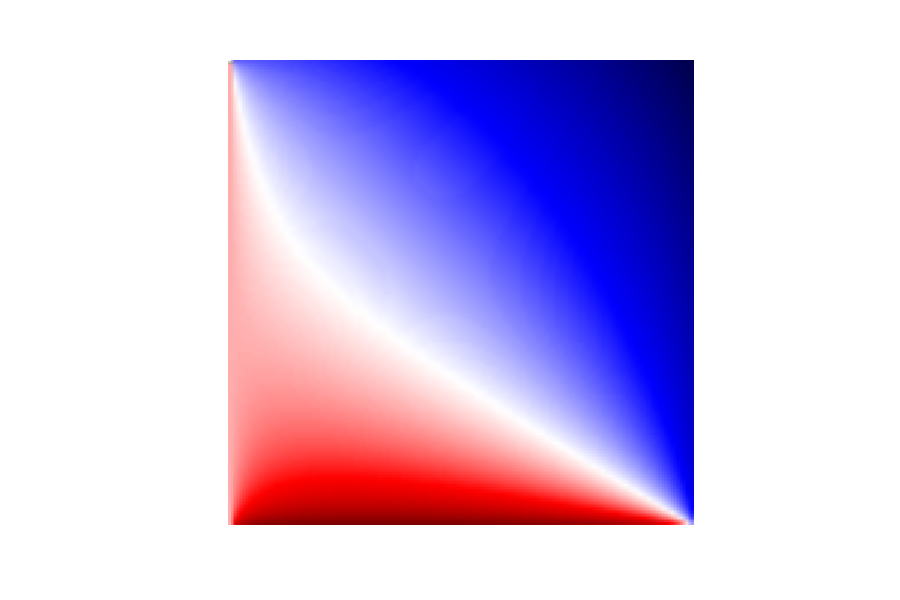
\includegraphics[width = 0.7\textwidth]{../img/WSLS-Analytical}}
    \caption{A comparison of a fingerprint plot from previous literature to asses the suitability of the Seismic colour map \cite{Ashlock2008}}
    \label{fig:WSLS-ashlock-comparison}
\end{figure}

With the knowledge that the choice of colour map is appropriate, a comparison can now be made between analytical fingerprints and numerical ones obtained via the Axelrod-Python library.
Table \ref{tab:fingerprint-functions} gives the analytical fingerprint functions of several well known strategies that will then be used to validate the numerical versions.

\begin{table}[htbp!]
\centering
\renewcommand{\arraystretch}{2}
\setlength{\tabcolsep}{12pt}
\begin{tabular}{l l}
\toprule
Strategy                 & Analytical Fingerprint Function\\
\midrule
TitForTat                & $\displaystyle \frac{y^2 + 5xy + 3x^2}{(x + y)^2} $\\
Psycho (Anti TitForTat   & $\displaystyle \frac{4(y-1)(x-1) + 5(y-1)^2}{2(y-1)(x-1) + (x-1)^2 + (y-1)^2} $ \\
WinStayLoseShit (Pavlov) & $\displaystyle \frac{(3x+y)(x-1) + 5y(y-1)}{(x+2y)(x-1) + y(y-1)} $\\
AllC (Cooperator)        & $\displaystyle 3 - 3y $ \\
AllD (Defector)          & $\displaystyle 4x + 1 $\\
\bottomrule
\end{tabular}
\caption{A selection of analytical fingerprint functions for well known strategies. The probe used is TitForTat.}
\label{tab:fingerprint-functions}
\end{table}

Figures \ref{fig:TFT-comparison} \ref{fig:Psycho-comparison}
\ref{fig:WSLS-comparison} \ref{fig:Cooperator-comparison} and \ref{fig:Defector-comparison} compare plots of known analytical fingerprint functions with numerical approximations obtained with the Axelrod-Python library.
The analytical plots were created with the code seen in listing \ref{lst:create-several-fingerprints}.
The parameters \mintinline{python}{turns=500, repetitions=200, step=0.01} are as described in section \ref{sec:fingerprint-implementation}.
The parameter \mintinline{python}{processes=0} ensures that the function will use the maximum number of cores available on the computer.

\begin{listing}[hbtp!]
\begin{ExampleCode}
import axelrod as axl
strats = [axl.TitForTat, axl.WinStayLoseShift, axl.AntiTitForTat,
          axl.Cooperator, axl.Defector]
for s in strats:
    probe = axl.TitForTat
    af = axl.AshlockFingerprint(s, probe)
    data = af.fingerprint(turns=500, repetitions=200, step=0.01, processes=0)
    p = af.plot()
    p.savefig('{}-Numerical.pdf'.format(s.name))
\end{ExampleCode}
\caption{Code to create the numerical plots for several strategies}
\label{lst:create-several-fingerprints}
\end{listing}

\begin{figure}[htbp!]
\subfloat[Exact analytical fingerprint]{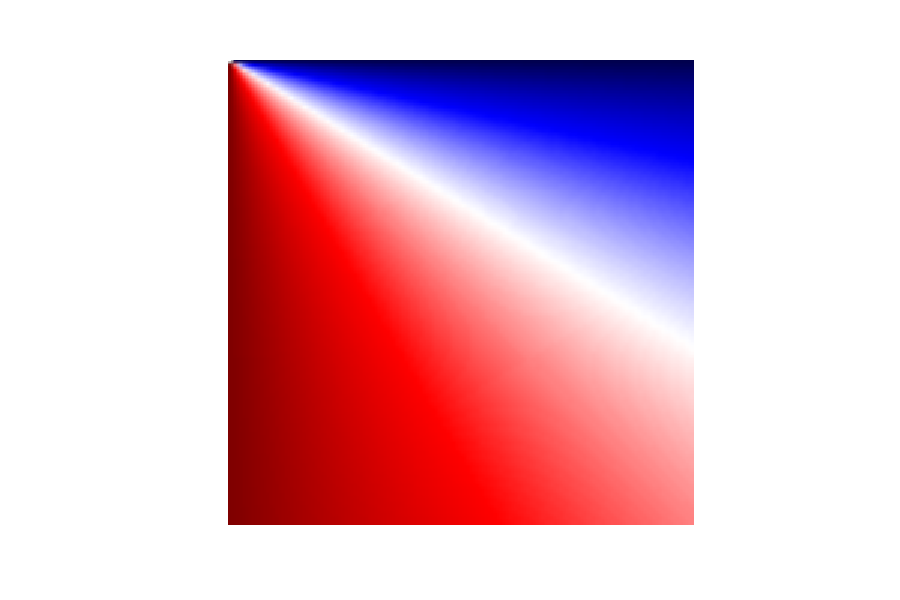
\includegraphics[width = 0.5\textwidth]{../img/TFT-Analytical.pdf}}
\subfloat[Numerical Fingerprint]{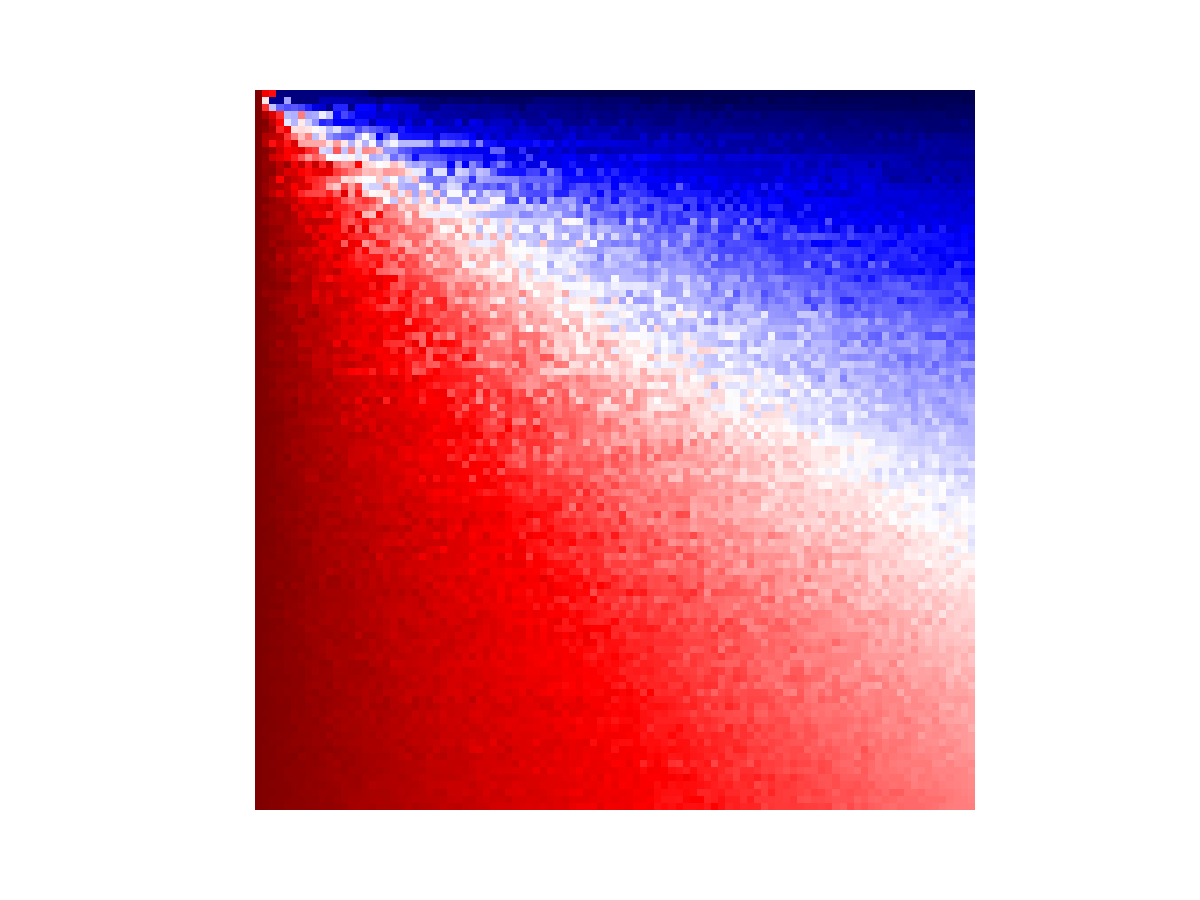
\includegraphics[width = 0.5\textwidth]{../img/Numerical/TitForTat.pdf}}
\caption{A comparison of the analytical fingerprint of TitForTat and the numerical version produced by Axelrod-Python library.}
\label{fig:TFT-comparison}
\end{figure}
\begin{figure}[htbp!]
\subfloat[Exact analytical fingerprint]{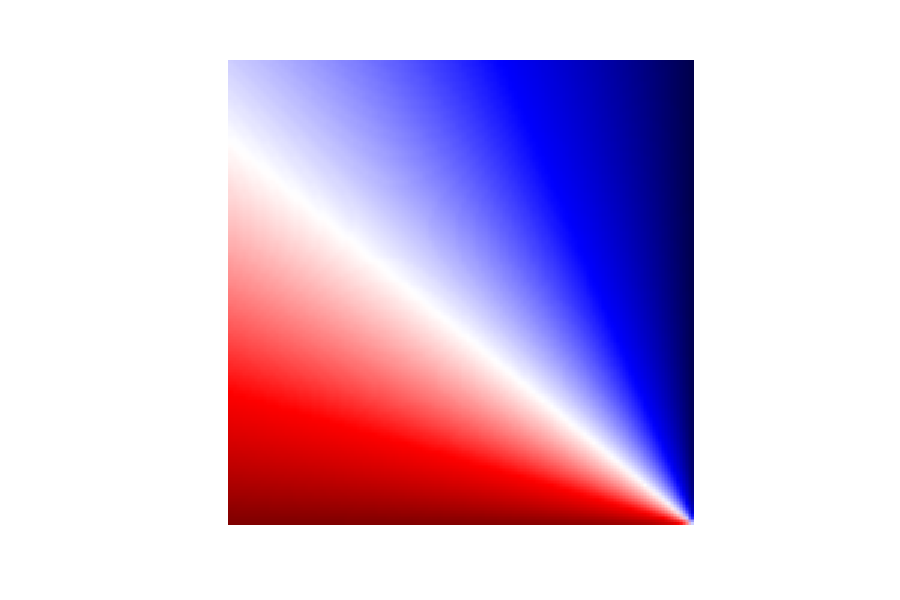
\includegraphics[width = 0.5\textwidth]{../img/Psycho-Analytical.pdf}}
\subfloat[Numerical Fingerprint]{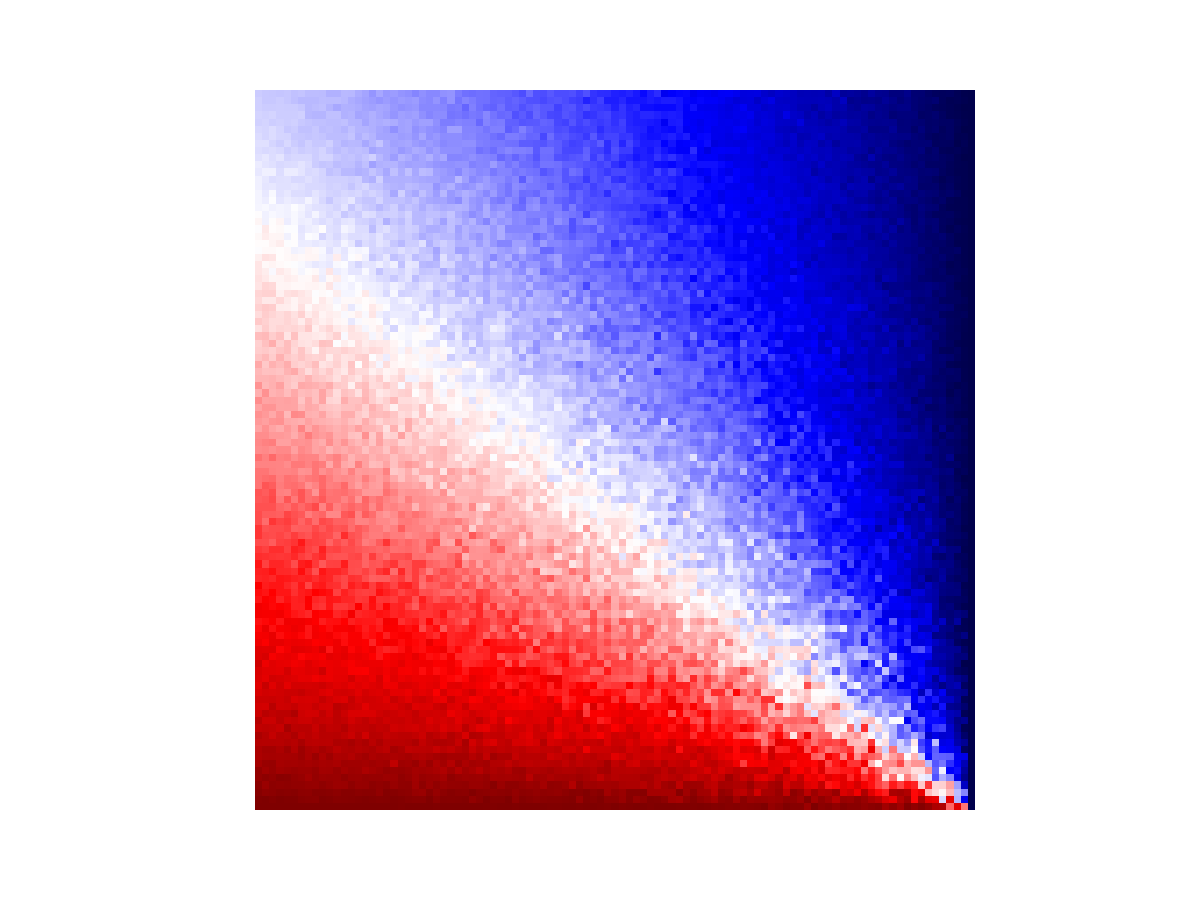
\includegraphics[width = 0.5\textwidth]{../img/Numerical/AntiTitForTat.pdf}}
\caption{A comparison of the analytical fingerprint of Psycho and the numerical version produced by Axelrod-Python library.}
\label{fig:Psycho-comparison}
\end{figure}
\begin{figure}[htbp!]
\subfloat[Exact analytical fingerprint]{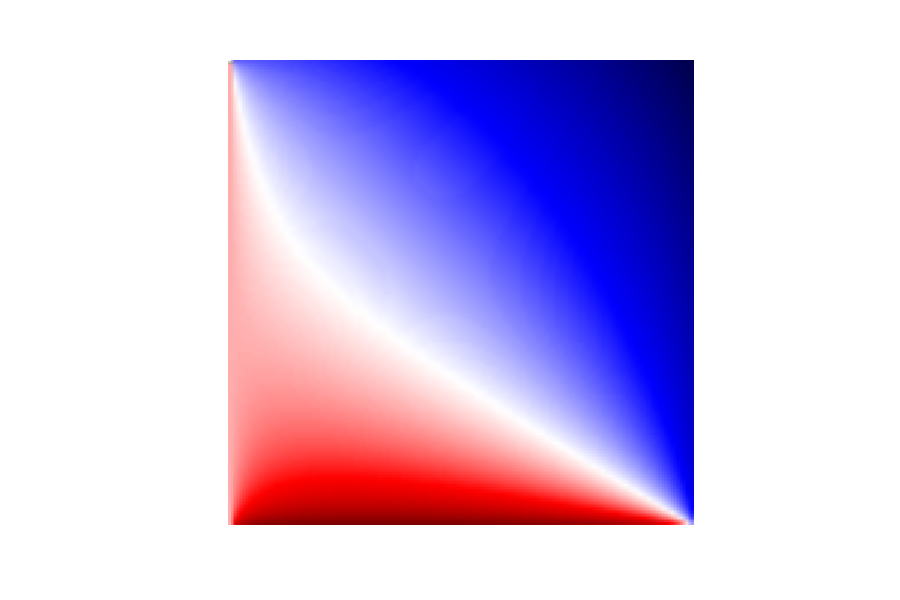
\includegraphics[width = 0.5\textwidth]{../img/WSLS-Analytical.pdf}}
\subfloat[Numerical Fingerprint]{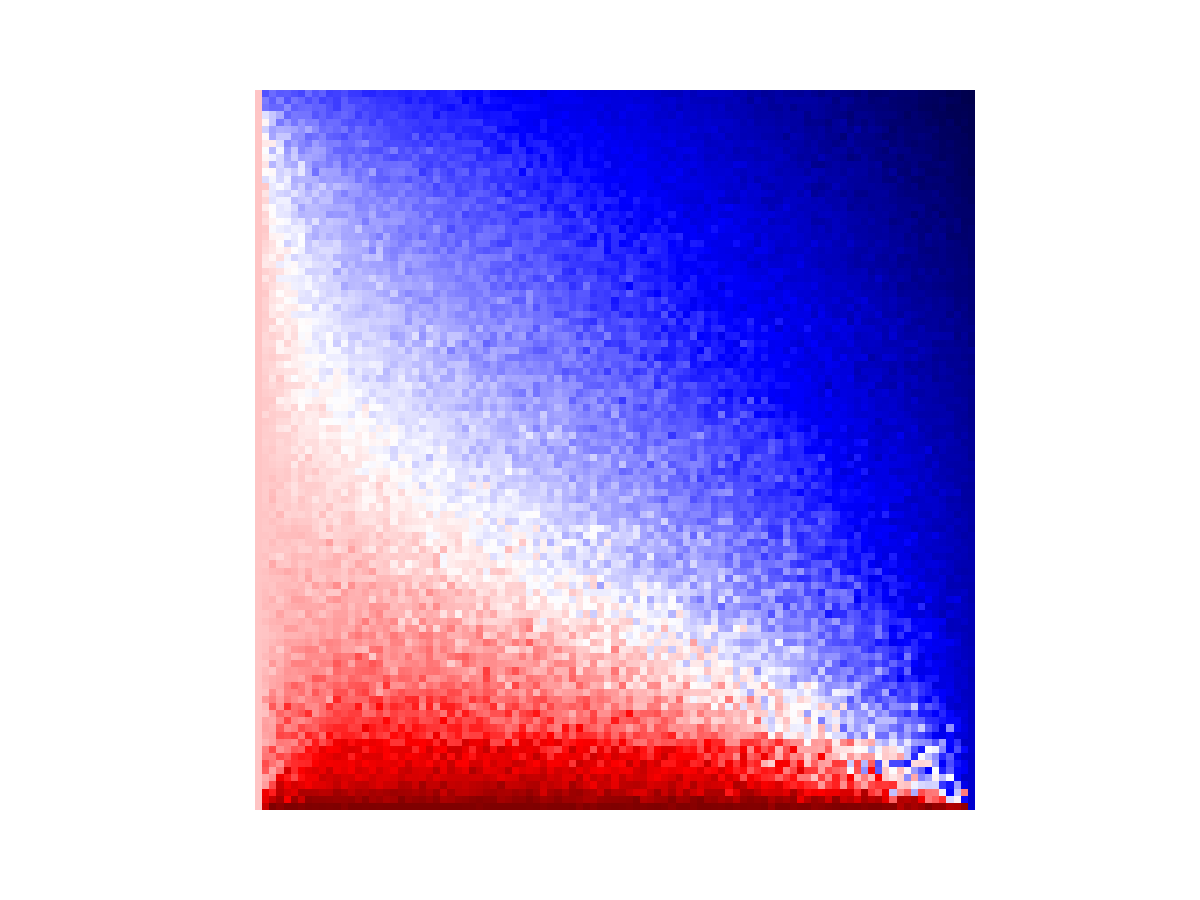
\includegraphics[width = 0.5\textwidth]{../img/Numerical/Win-Stay-Lose-Shift.pdf}}
\caption{A comparison of the analytical fingerprint of WinStayLoseShit and the numerical version produced by Axelrod-Python library.}
\label{fig:WSLS-comparison}
\end{figure}
\begin{figure}[htbp!]
\subfloat[Exact analytical fingerprint]{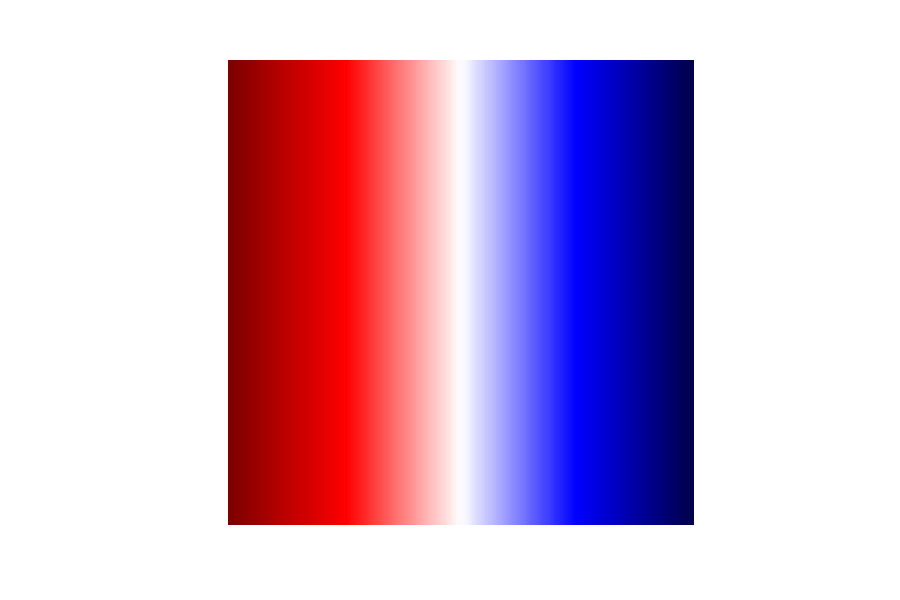
\includegraphics[width = 0.5\textwidth]{../img/AllC-Analytical.pdf}}
\subfloat[Numerical Fingerprint]{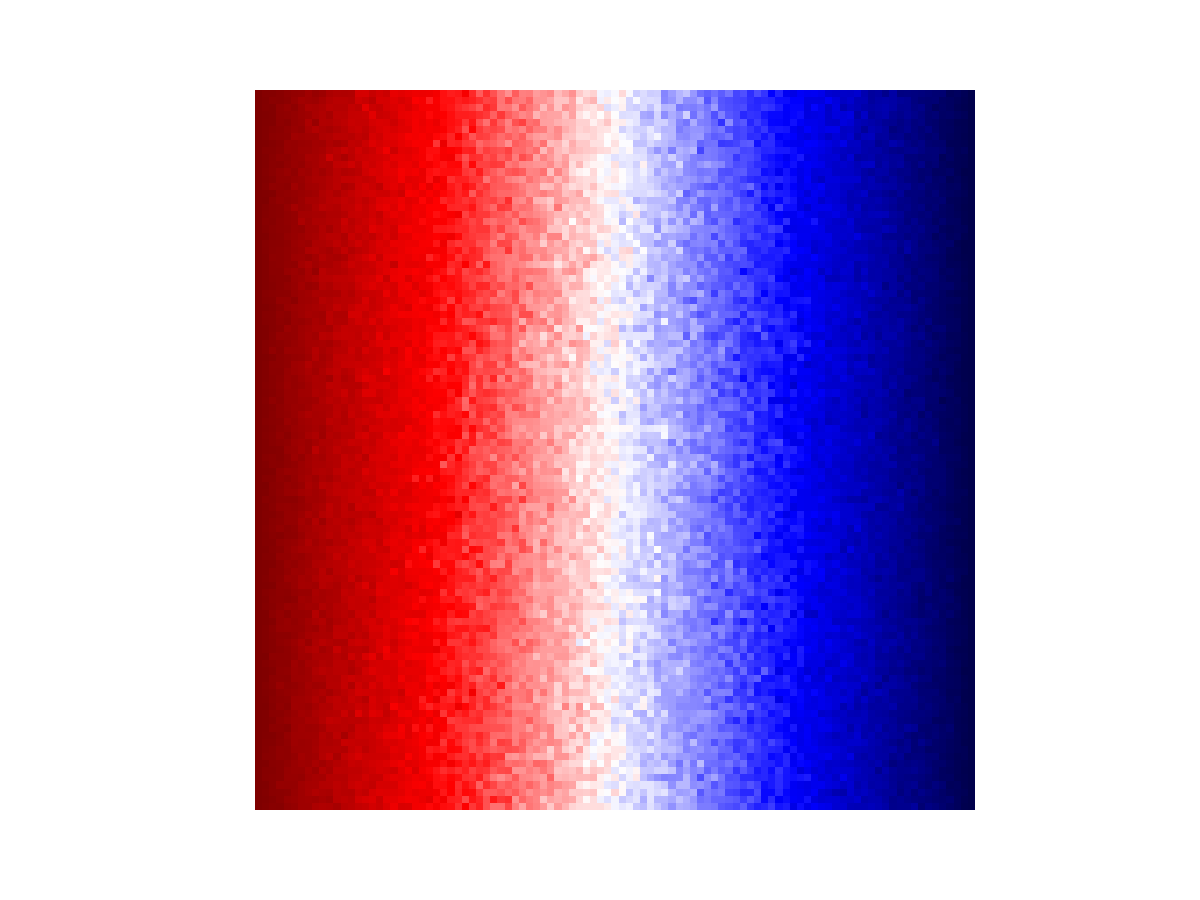
\includegraphics[width = 0.5\textwidth]{../img/Numerical/Cooperator.pdf}}
\caption{A comparison of the analytical fingerprint of Cooperator and the numerical version produced by Axelrod-Python library.}
\label{fig:Cooperator-comparison}
\end{figure}
\begin{figure}[htbp!]
\subfloat[Exact analytical fingerprint]{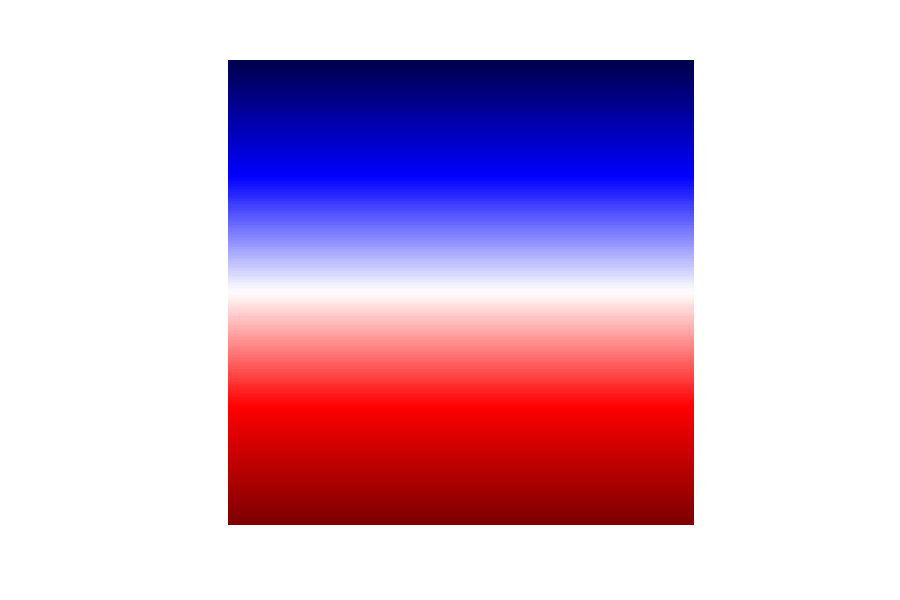
\includegraphics[width = 0.5\textwidth]{../img/AllD-Analytical.pdf}}
\subfloat[Numerical Fingerprint]{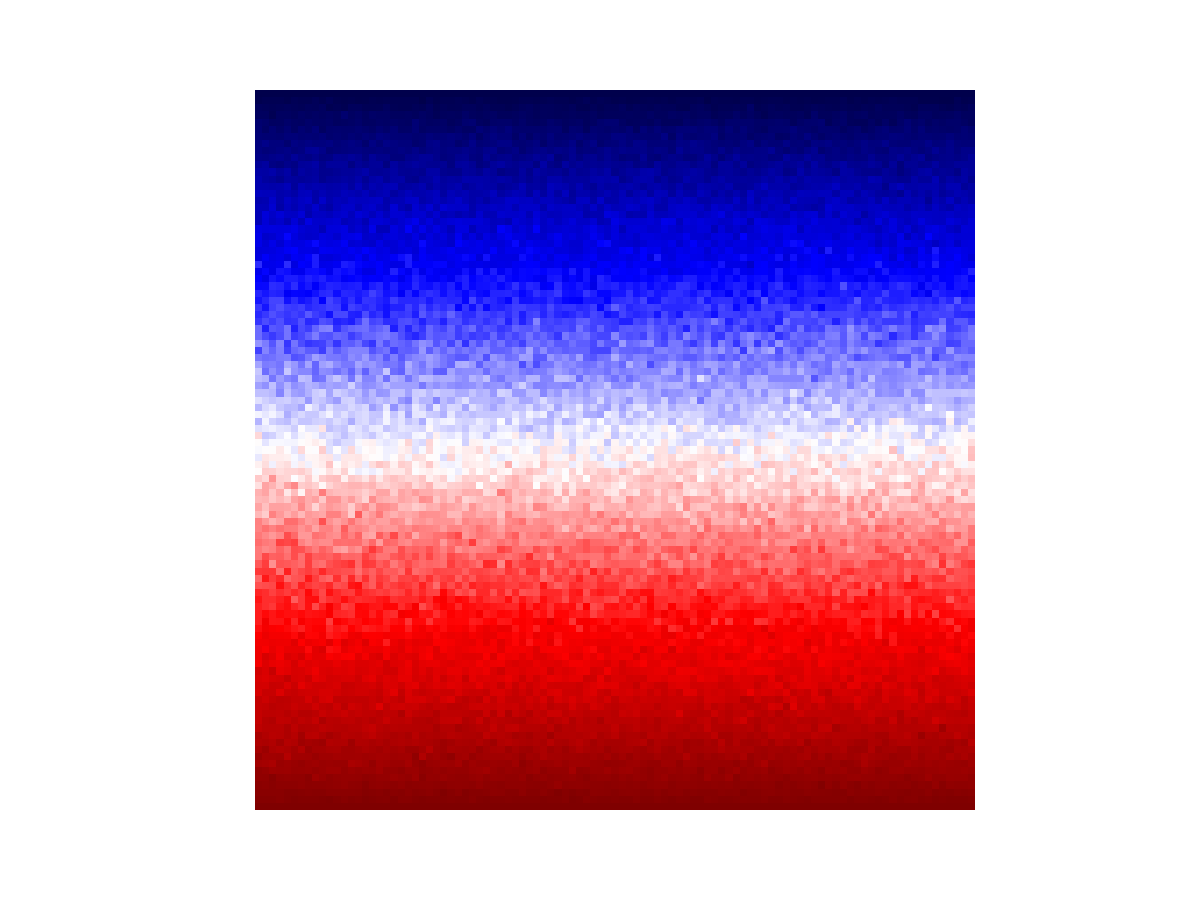
\includegraphics[width = 0.5\textwidth]{../img/Numerical/Defector.pdf}}
\caption{A comparison of the analytical fingerprint of Defector and the numerical version produced by Axelrod-Python library.}
\label{fig:Defector-comparison}
\end{figure}

\section{The Development Process}\label{sec:dev_process}

The Axelrod-Python library aims to follow best practice at all times with regards to development.
This section outlines some of these key ideas, and how they were relevant to the implementation of the ability to produce fingerprints within Axelrod-Python.

\subsection{Version Control}
Scientists face many issues when producing research in the modern world.
One of the main reasons research can be hard to reproduce is due to the lack of access to underlying data and code, which reduces the opportunity for others to verify findings \cite{Schwab2000, Ince2012}.
Also, two of the biggest challenges scientists and other programmers face when working with code and data are keeping track of changes (and being able to revert them if things go wrong), and collaborating on a program or dataset \cite{Wilson2013, Matthews}.
Both of these issues can be resolved by ensuring that all code is version controlled.

Version control systems give users the ability to save versions of files during development along with informative comments which are referred to as commit messages.
Every change and accompanying notes are stored independent of the files.
Commits serve as checkpoints where individual files or an entire project can be safely reverted to when necessary \cite{Ram2013}.
Version control ensures that all changes to a code base are tracked and can be traced back to a particular author.
There are many version control systems available and Axelrod-Python uses Git \cite{Git} with all code hosted at Github.
One of the major benefits is that every repository (including the one on Github) contains the entire history of all changes, including authorship, and can be viewed by anyone.

\subsection{Review Process}
The library also applies a strict review process, where any code submission is analysed by several members of the organisation before it can be included.
This normally involves other developers requesting changes to the submission, this ensure that all source code is of the same high standard.
Figures \ref{fig:screenshot1} to \ref{fig:screenshot4} shows some screen shots of the discussions, requests and suggestions made during the development process of the fingerprint code.

\begin{figure}[htbp!]
\centering
\includegraphics[width = \textwidth]{../img/screenshots/ScreenShot1.png}
\caption{A refactoring suggestion to create a new function to avoid repetition}
\label{fig:screenshot1}
\end{figure}

\begin{figure}[htbp!]
\includegraphics[width = \textwidth]{../img/screenshots/ScreenShot4.png}
\caption{Suggestion to move some code to the module level so that it is more accessible}
\label{fig:screenshot2}
\end{figure}

Figures \ref{fig:screenshot1} and \ref{fig:screenshot2} show suggestions that have been made.
These suggestions do not highlight errors within the code, but are merely small recommendations from experienced developers for ways to improve.

\begin{figure}[htbp!]
\includegraphics[width = \textwidth]{../img/screenshots/ScreenShot2.png}
\caption{Advice to use other code being developed for the library}
\label{fig:screenshot3}
\end{figure}

Figure \ref{fig:screenshot3} is an example of the power of using git.
Code that is being developed elsewhere can still be used as part of this project, even though it is not yet available as part of the standard library.
This is a common occurrence when developing software; some code may rely on other parts but they are not being written by the same person.

\begin{figure}[htbp!]
\includegraphics[width = \textwidth]{../img/screenshots/ScreenShot3.png}
\caption{Request to remove redundant lines of code}
\label{fig:screenshot4}
\end{figure}

Figure \ref{fig:screenshot4} is a request to move unnecessary lines of code.
Whilst these would not cause the software to break, it is bad coding practice to have unused imports and redundant lines of code.
This is an example of something that would have prevented the code written from being included in the production version of the package.

\subsection{Testing}
All code in Axelrod-Python must be tested and the most common example of testing is unittesting.
A unit test is a function that tests a small pieces of code and not an entire package/module, although it sometimes can.
They operate by observing the result for a specific input and comparing it with a known output, then returning whether they are the same.
A result of True indicates that the code is behaving as intended, and a result of False indicates that it is not.
Consequently any program relying on that code cannot be trusted to behave as intended \cite{Sarma2016, Williams}.

Axelrod-Python uses several external programmes to help with testing.
Travis \cite{Travis} provides continuous integration testing, so all tests are run automatically whenever any changes to code are made.
% TODO Add a screenshot of all the tests passing on the PR?
Coveralls \cite{Coveralls} calculates what proportion of the code is tested, and can highlight areas that are either untested or need improvement.
Finally, Hypothesis \cite{Hypothesis3.6.1} is a library for property testing.
It works by generating random data matching a specification and checking that a specified guarantee still holds in that case.
If it finds an example where it doesn’t, it takes that example and cuts it down to size, simplifying it until it finds a much smaller example that still causes the problem \cite{HypothesisDocs}.
% TODO Do you want to add something about documentation and doctesting too?
% TODO Needs a conclusion etc (what was the version of Axelrod that first had
% fingerprinting: check the twitter feed or CHANGES.md)
